\documentclass[11pt]{article}
\usepackage[latin2]{inputenc}
\usepackage{a4wide}
\usepackage{graphicx}
\title{Prusa Mendel documentation}
\author{ThingDOC.py}
\begin{document}
\maketitle
Prusa Mendel is machine from RepRap project. RepRap is open source 3D printer.
\newpage
\tableofcontents
\newpage
\section{Bill of materials}
List of things you need to build the machine devided by categories
\subsection{Printed}
\begin{itemize}
\item 8x Bar clamp
\item 4x Belt clamp
\item 2x Coupling
\item 3x Endstop holder
\item 2x Frame vertex
\item 4x Frame vertex with foot
\item 2x Frame vertex
\item 4x Frame vertex with foot
\item 8x Bushing
\item 8x Bushing
\item 2x Pulley
\item 2x Rod clamp
\item 1x X carriage
\item 1x X end idler
\item 1x X end motor
\item 1x Y motor bracket
\item 2x Z motor mount
\end{itemize}
\subsection{Nuts\&bolts}
\begin{itemize}
\item 72x M8 nut
\item 68x M8 washer
\item 2x M8 spring
\item 19x M3 nut
\item 25x M3 washer
\item 17x M3 10mm screw
\item 3x M3 20mm screw
\item 6x M3 25mm screw
\end{itemize}
\newpage
\section{Things overview}
List of things and their descriptions
\subsection{Frame vertex}


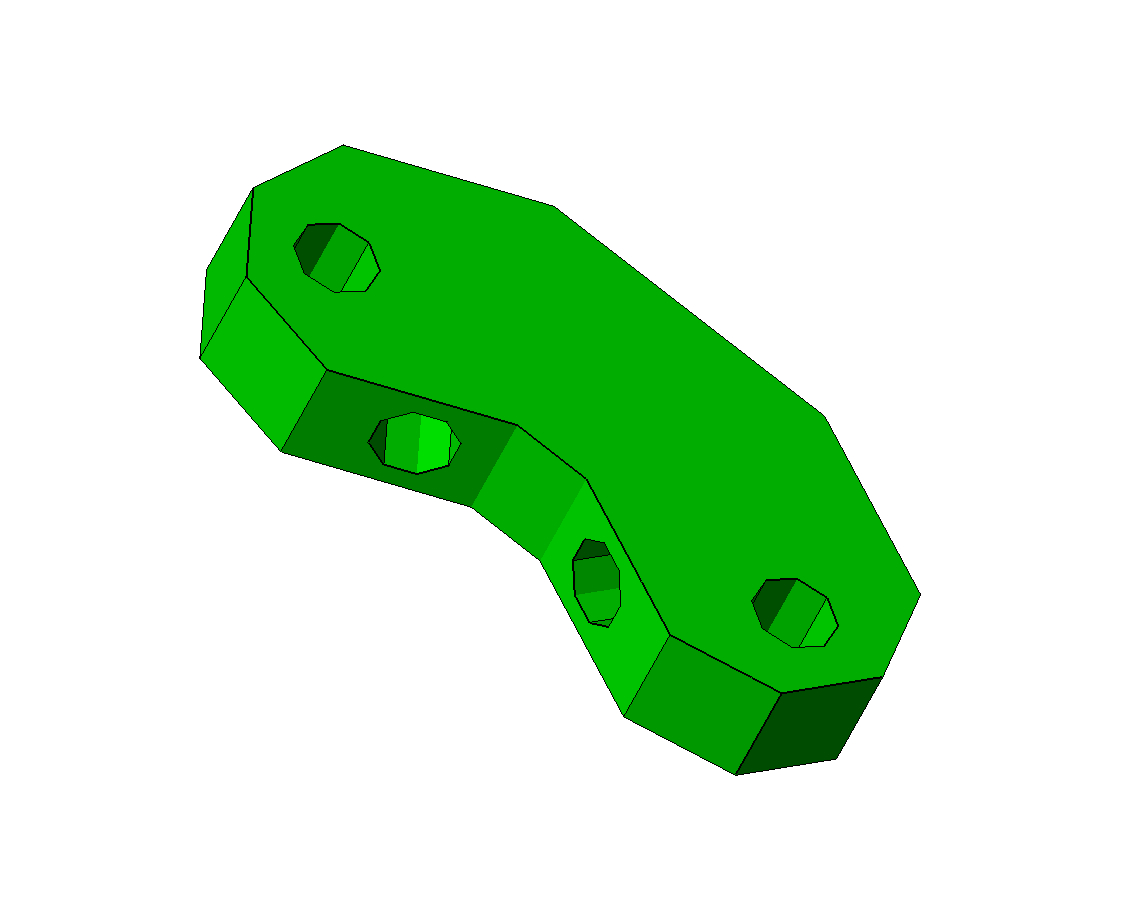
\includegraphics[width=4cm]{images/frame-vertex.jpg}
\subsection{Frame vertex}


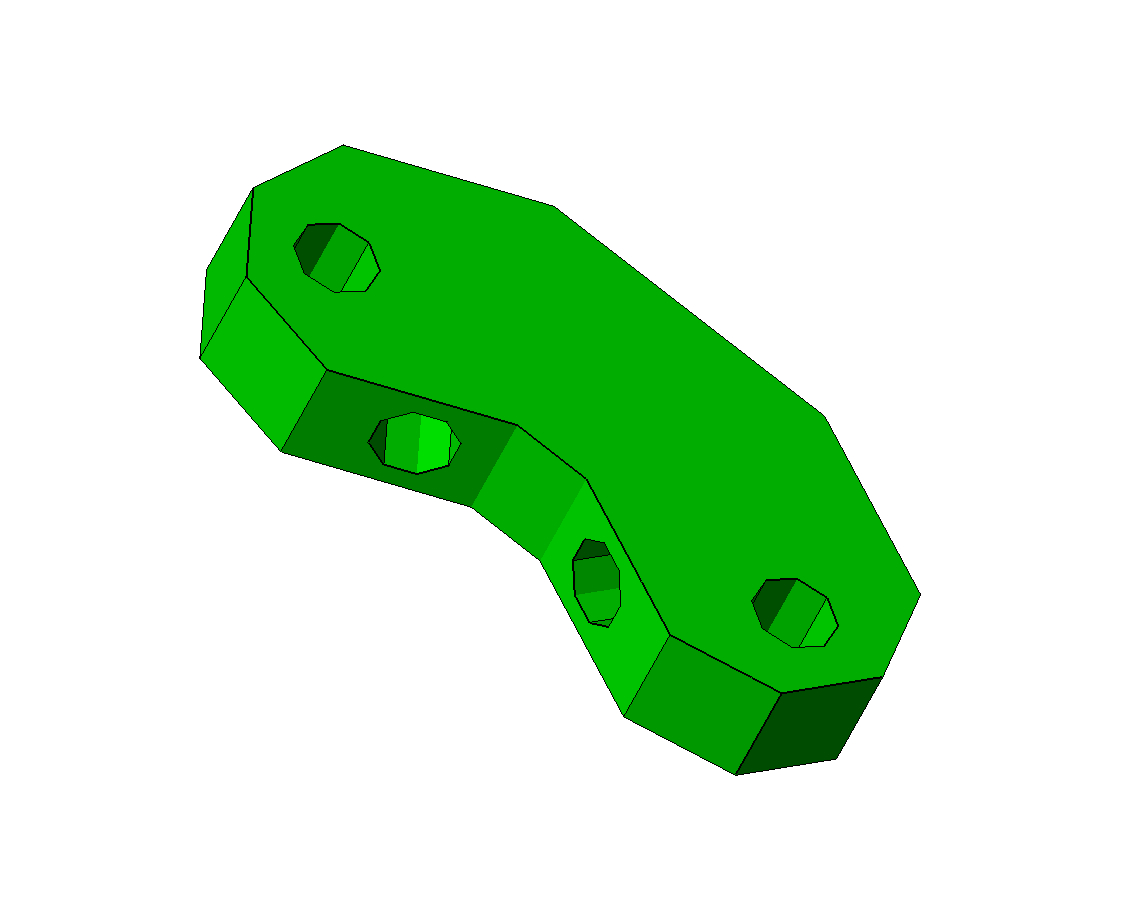
\includegraphics[width=4cm]{images/frame-vertex.jpg}
\subsection{Frame}
Frame for adding all of the other parts

\subsection{Y motor bracket}


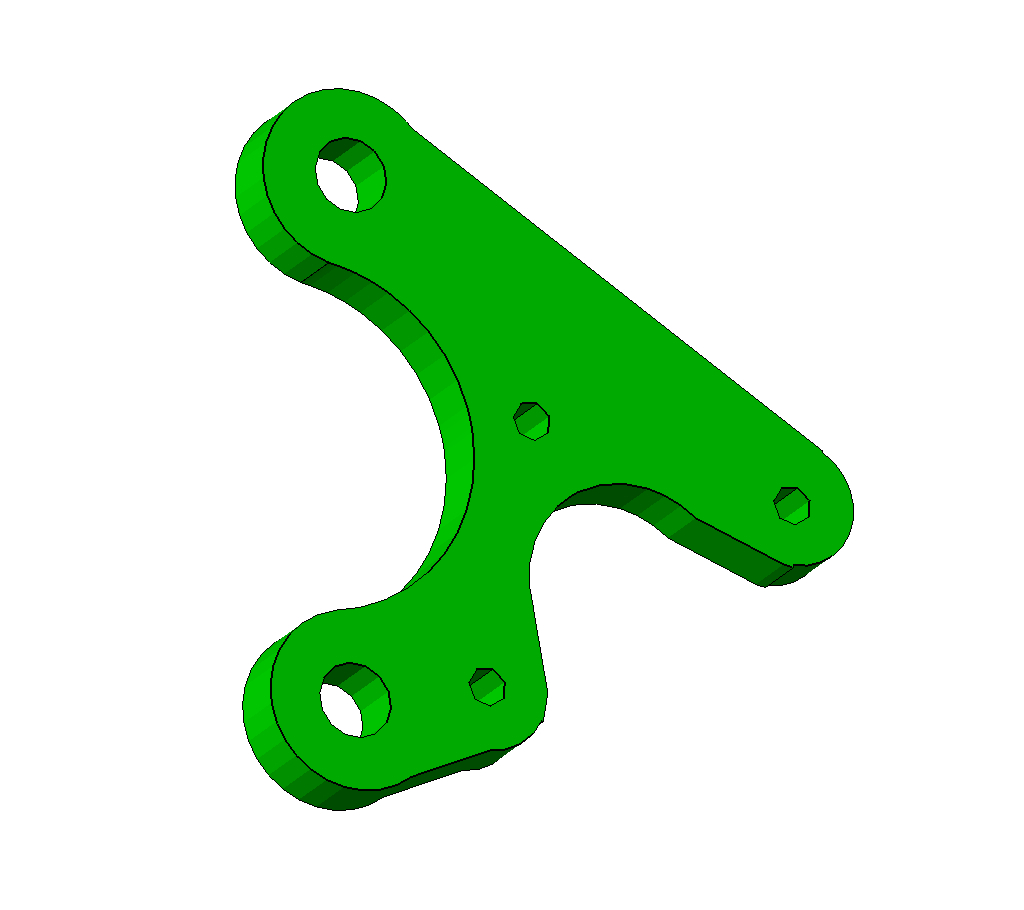
\includegraphics[width=4cm]{images/y-motor-bracket.jpg}
\subsection{Belt clamp}


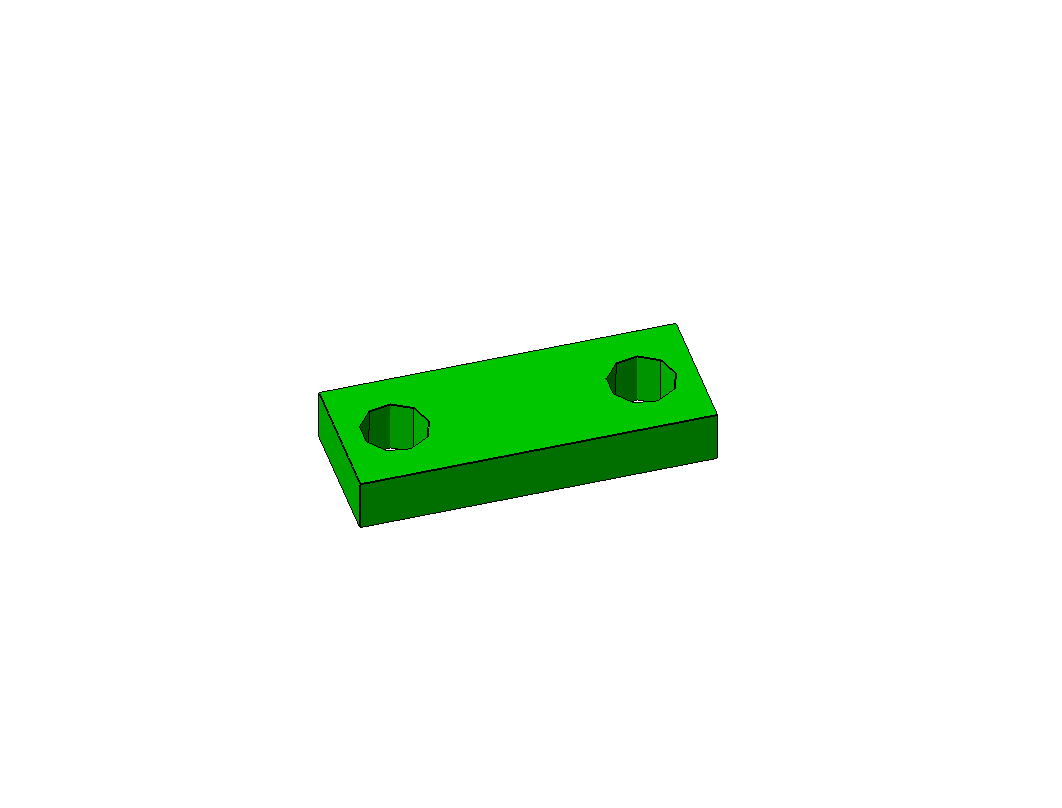
\includegraphics[width=4cm]{images/belt-clamp.jpg}
\subsection{Bar clamp}


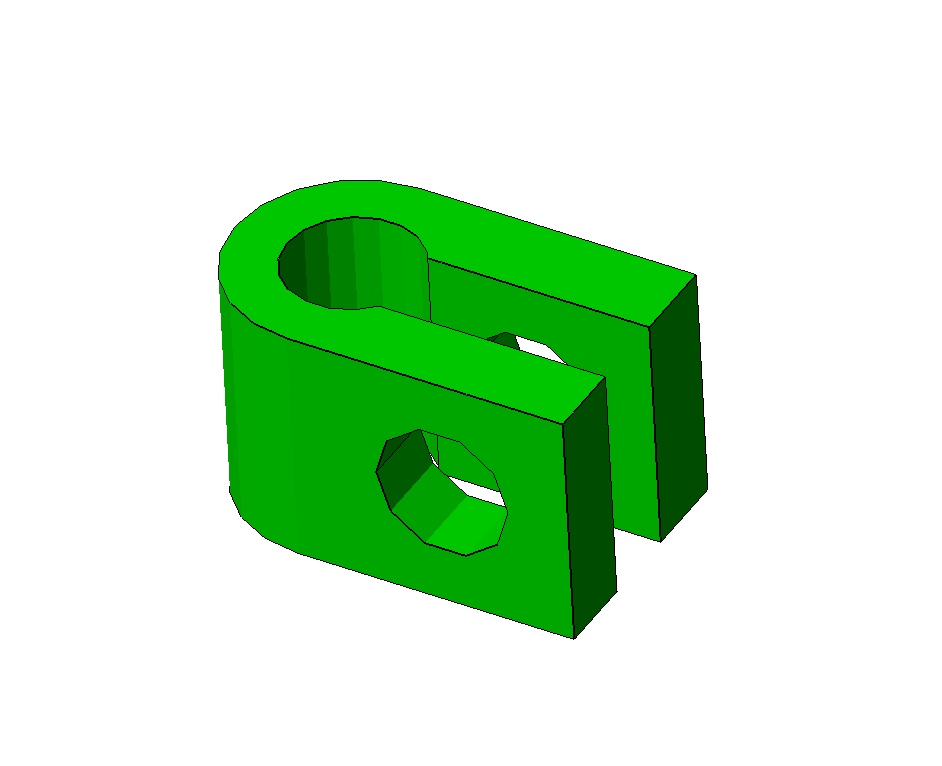
\includegraphics[width=4cm]{images/bar-clamp.jpg}
\subsection{Frame vertex with foot}


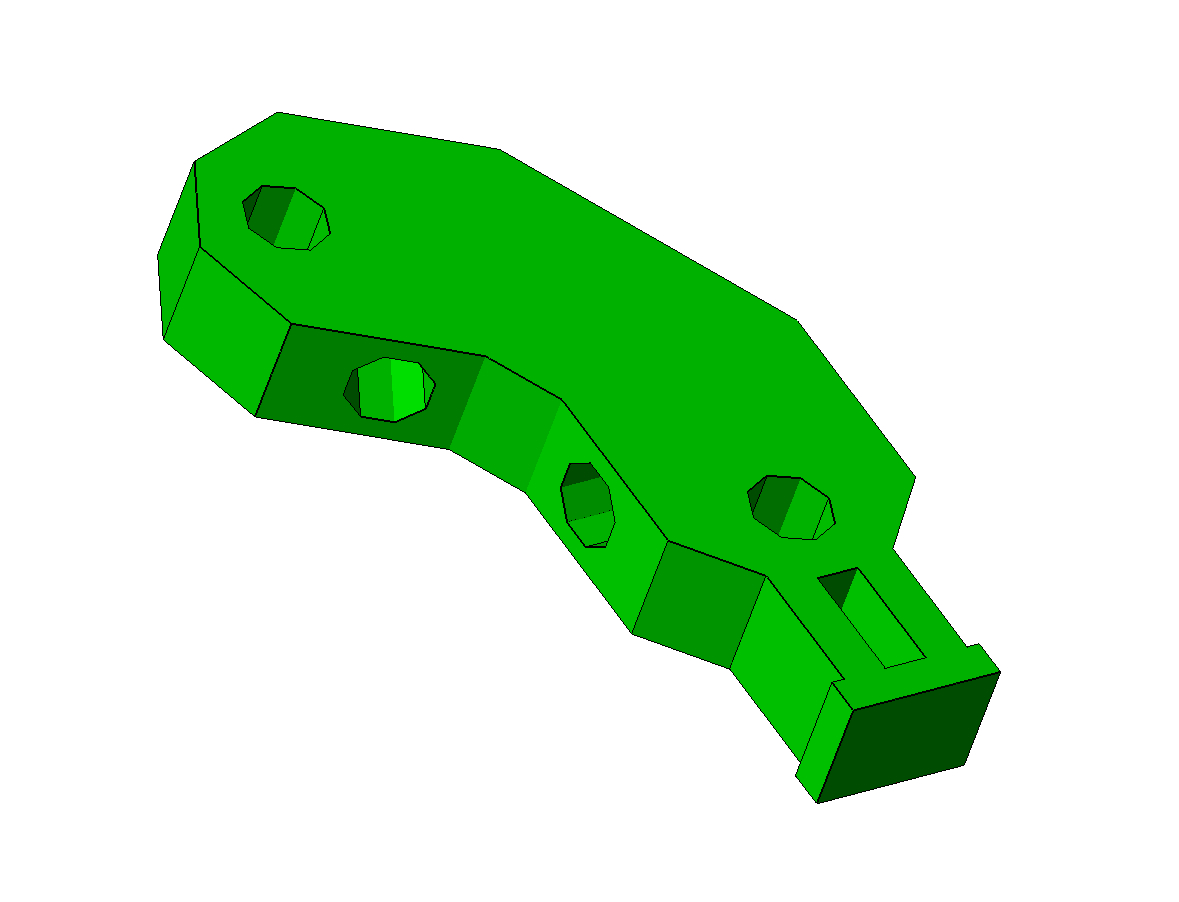
\includegraphics[width=4cm]{images/frame-vertex-foot.jpg}
\subsection{Frame vertex with foot}


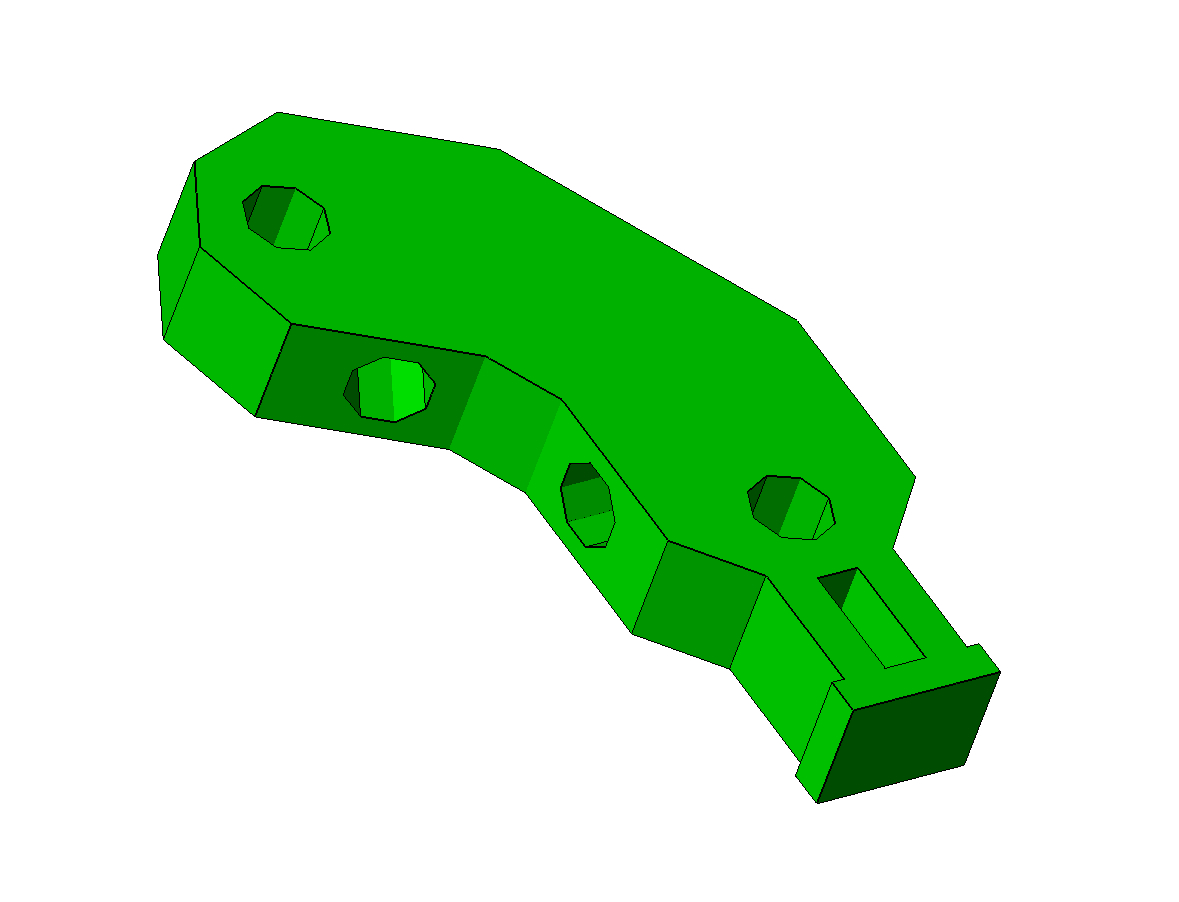
\includegraphics[width=4cm]{images/frame-vertex-foot.jpg}
\subsection{Z motor mount}


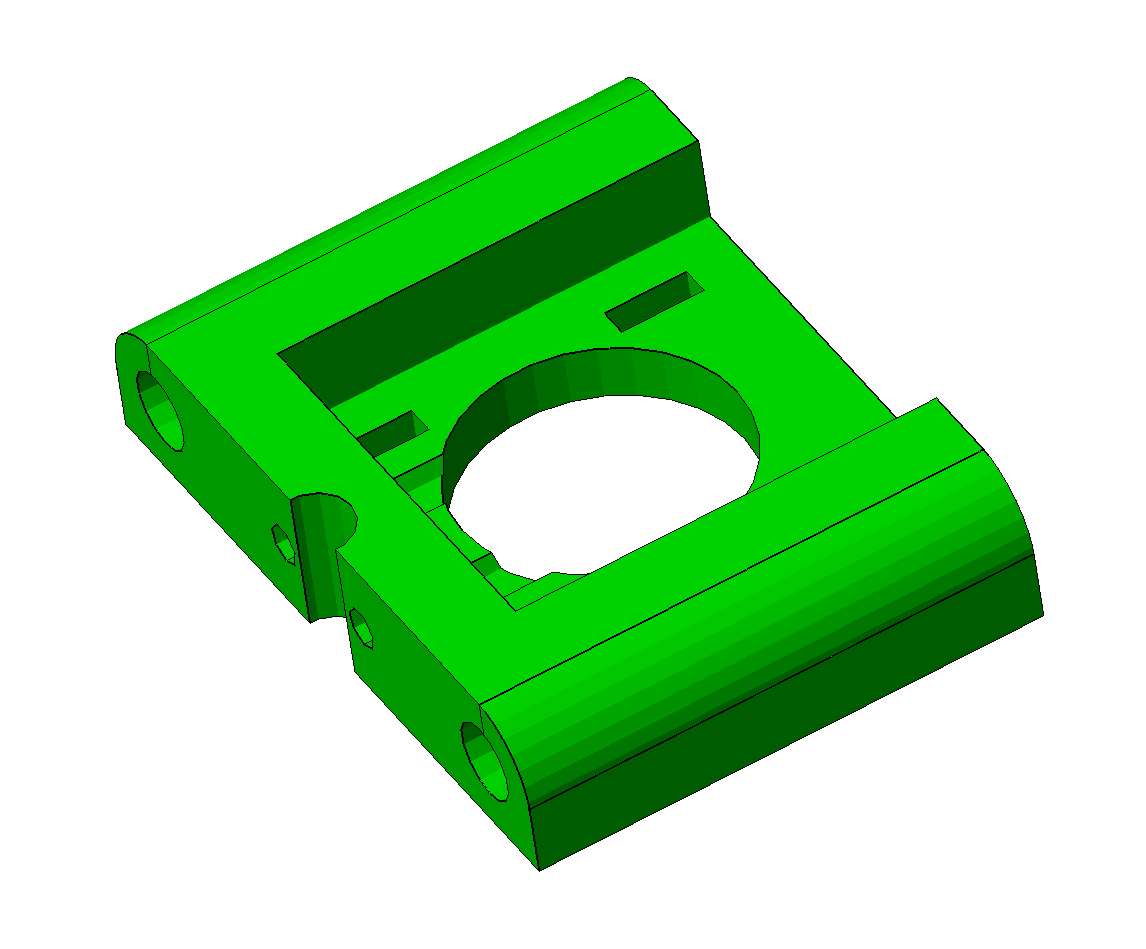
\includegraphics[width=4cm]{images/z-motor-mount.jpg}
\subsection{X end idler}


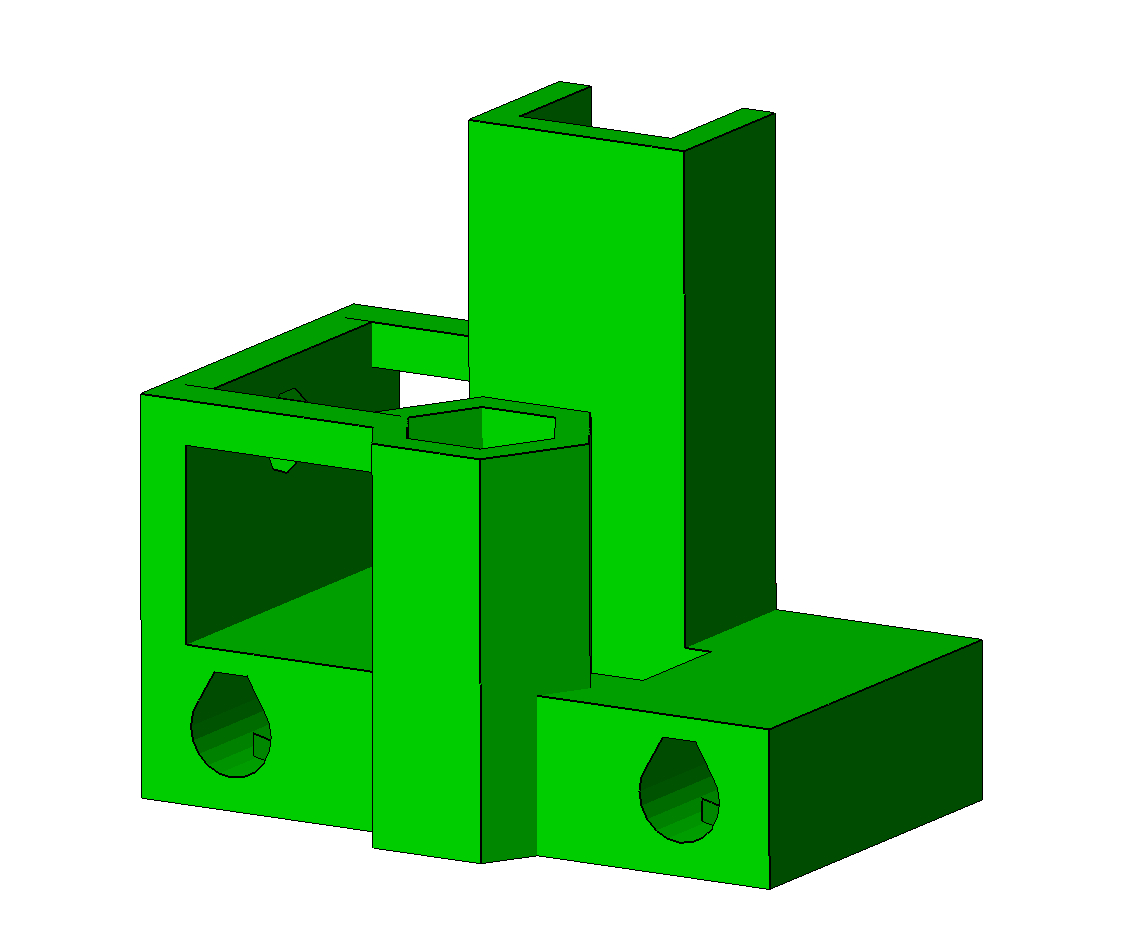
\includegraphics[width=4cm]{images/x-end-idler.jpg}
\subsection{Endstop holder}


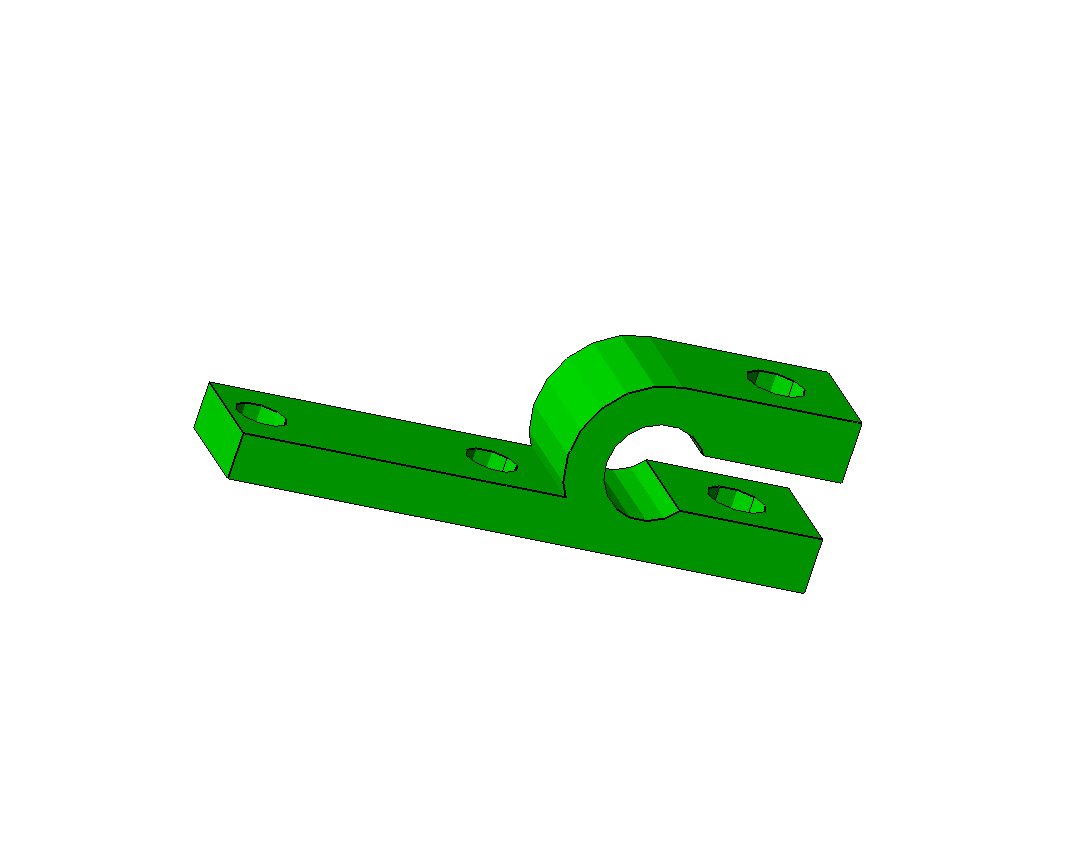
\includegraphics[width=4cm]{images/endstop-holder.jpg}
\subsection{Rod clamp}


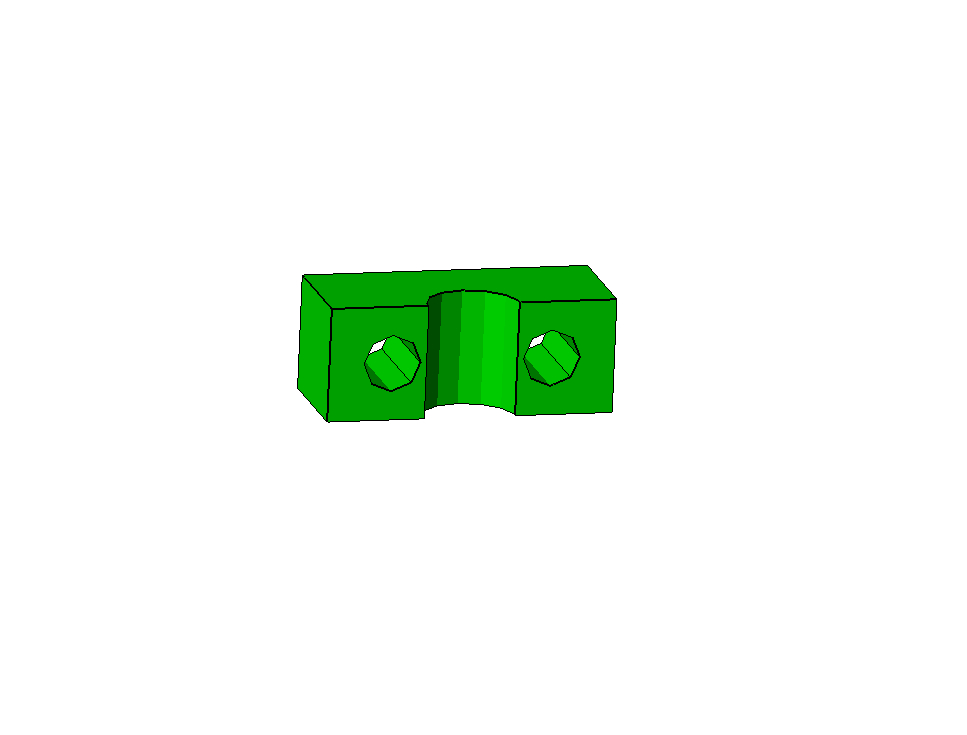
\includegraphics[width=4cm]{images/rod-clamp.jpg}
\subsection{Bushing}


\subsection{Bushing}


\subsection{X carriage}
Slides on the x-axis with extruder.

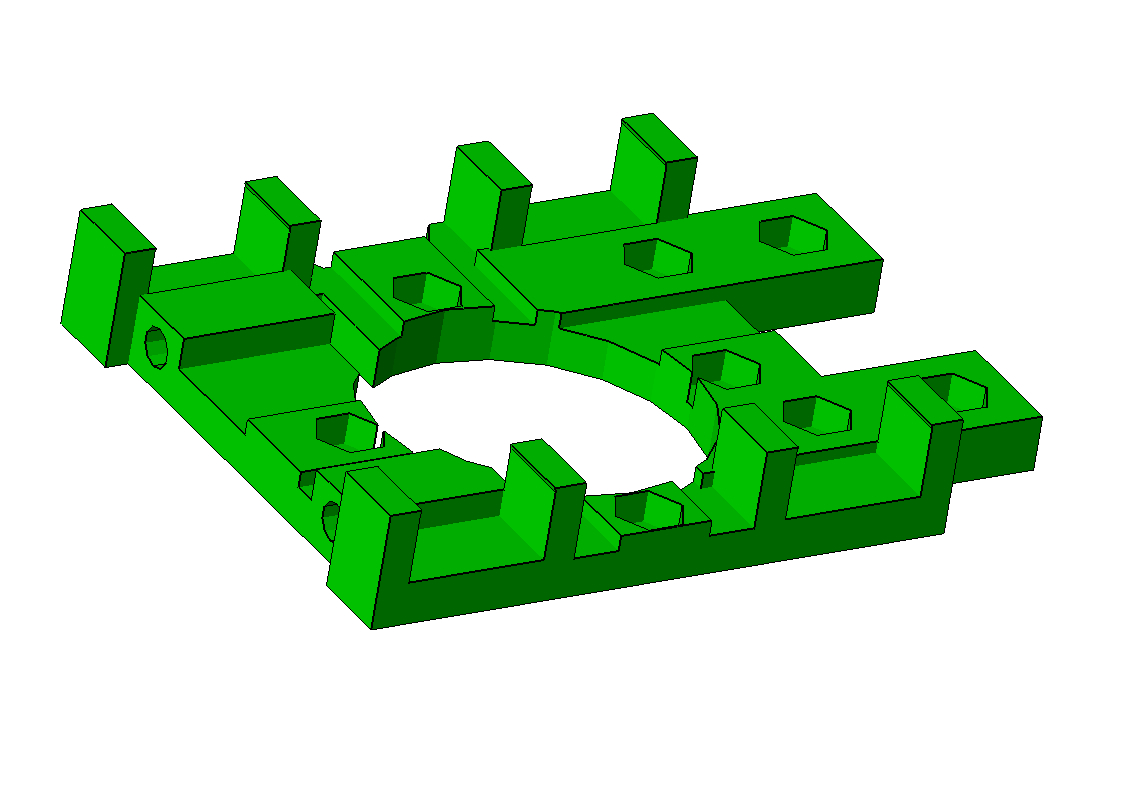
\includegraphics[width=4cm]{images/x-carriage.jpg}
\subsection{Pulley}


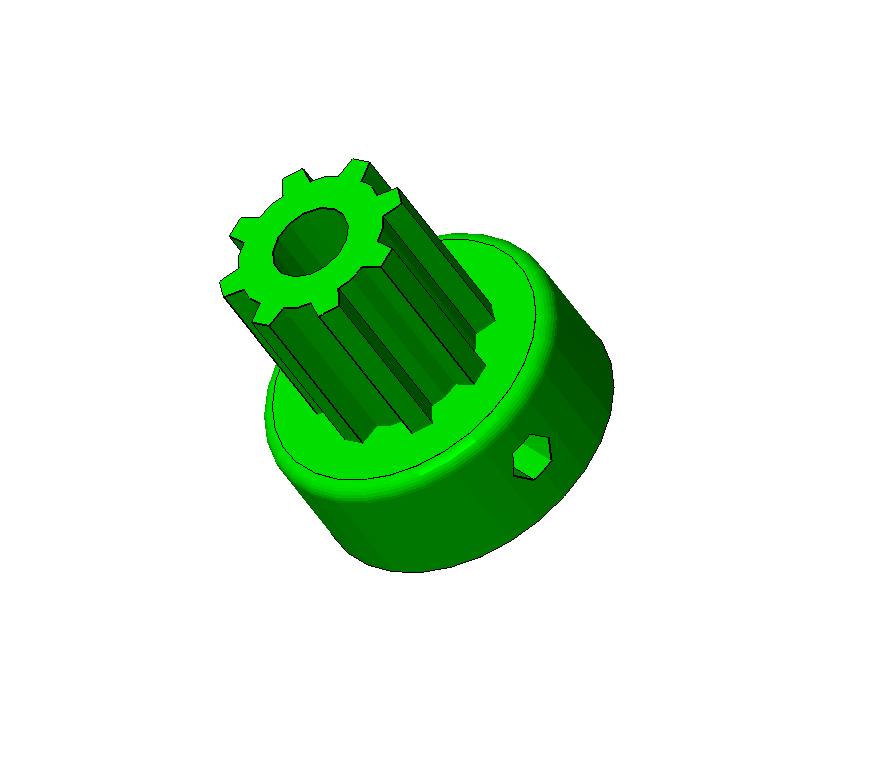
\includegraphics[width=4cm]{images/pulley.jpg}
\subsection{Coupling}


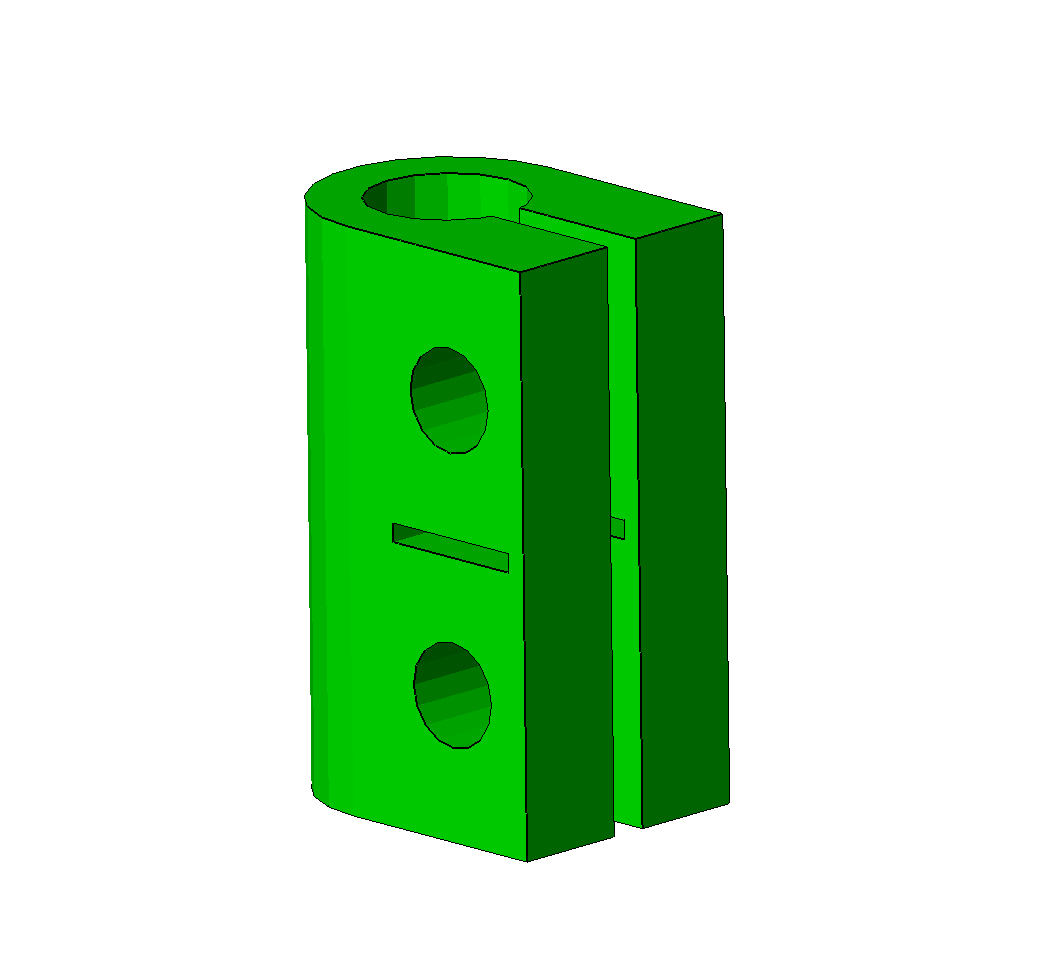
\includegraphics[width=4cm]{images/coupling.jpg}
\subsection{X end motor}


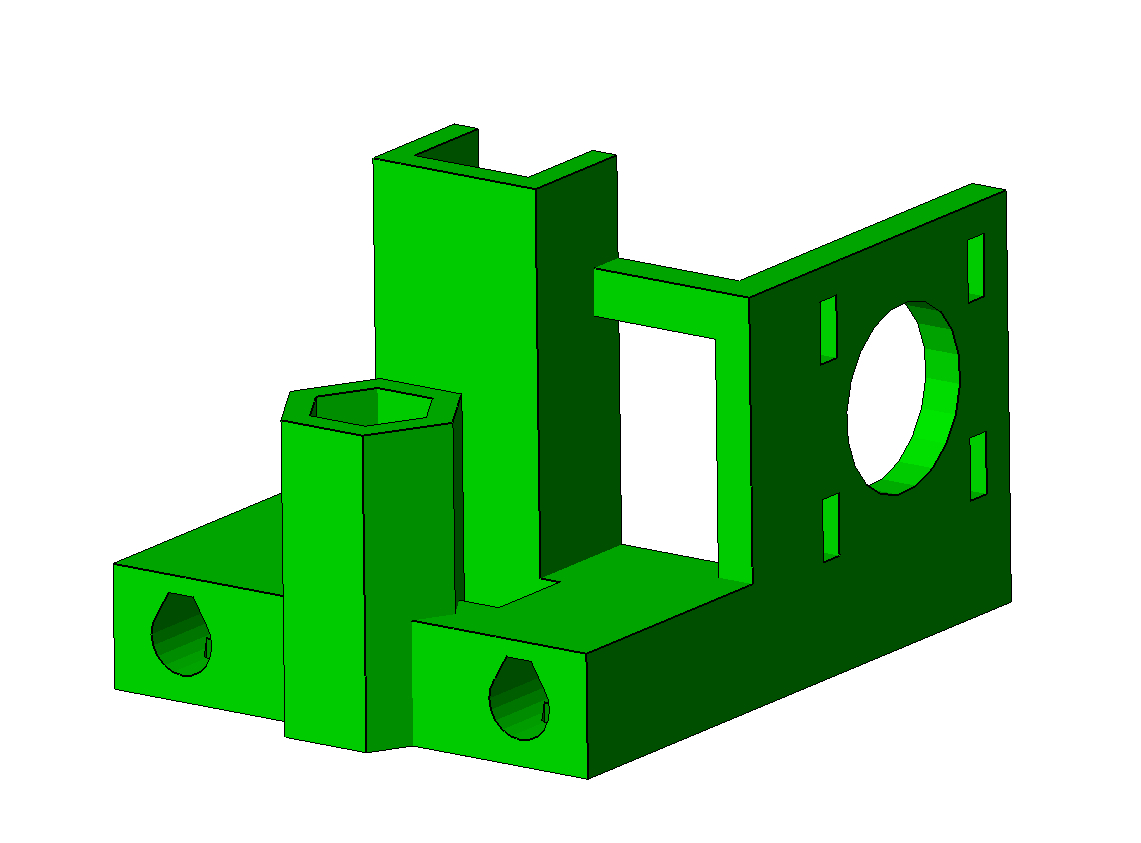
\includegraphics[width=4cm]{images/x-end-motor.jpg}
\newpage
\section{Assembly Instructions}
Instructions to assemble the machine
\subsection{Assemble Prusa Mendel}
\begin{itemize}
\item Assembly info
\end{itemize}
\end{document}
